\chapter{Elméleti háttér} \label{theoryChapter}

Ahhoz, hogy kellőképpen megértsük a dolgozat által felvetett problémákat, úgy gondolom, hogy szükséges azokat megfelelően, matematikailag tisztán megalapozni. Célom precízen kimondani a megoldandó problémákat, valamint a rájuk alkalmazott különféle technikákat.

\section{Utazóügynök probléma \label{TSPsection}}

Az utazóügynök probléma (Travelling Salesman Problem - TSP)  egy optimalizációs feladat, mely során egy utazónak minél rövidebb úton kell megtennie körutat egy adott ponthalmazon. 

Precízen fogalmazva: Adott a bemeneten egy G=(V,E) (irányított) gráf, \[n = |V(G)|, n > 2 \] az állomások száma (a kiindulási állomást beleértve),  \[m = |E(G)| \] az állomások között futó elérhető utak száma.

\[ V = (v_0,v_1, \dots v_n )\]  állomások halmaza (Vertex), \(0 \in V\) a kiindulási állomás,
\[ E = (e_1,e_1, \dots e_m)\] elérhető utak halmaza (Edge),
\[ D : E(G) \mapsto \mathbb{Z}^+\] költségfüggvény (Distance).

A kimenet a legkisebb költségű Hamilton-kör G-re, vagyis azon 
\[ R = (0, v_{i0}, v_{i1} ... 0) \]
bejárás, hogy \( \forall v_i \in V, v_i \in R \) mindegyik csúcsot tartalmazza, és költsége minimális \cite{alg_optim}.

\begin{figure}[ht!]
	\centering
	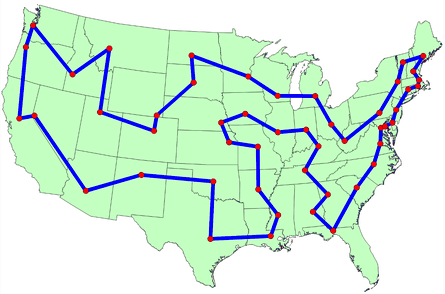
\includegraphics[width=0.5\textwidth]{figures/tsp-usacities.png}
	\caption{Egy példa TSP végrehajtására az USA szárazföldi államai fővárosának körbeutazása \label{TSPpelda} \cite{TSPimage} }
\end{figure}

A téma a nevét onnan kapta, hogy a XX. században utazó porszívóügynökök autóval járták az Egyesült Államok útjait kereskedés céljából. Az olajválság során megdrágult a járművek működtetéséhez szükséges üzemanyag, és hirtelen megnőtt az igény arra, hogy minél jobban minimalizálják a megtett út hosszát egy-egy üzleti út során. A problémának azóta több alkalmazása is lett, ebből a villamosmérnöki gyakorlathoz egyik legközelebb az SMD beültetőgép bejárása áll. A gép feladata, hogy egy adott nyomtatott áramköri terv alapján lepakolja az alkatrészeket a hordozó lapkára. Az iparban fontos a sebesség, ugyanis ha felére csökkentjük a beültetési időt, akkor akár duplaannyi terméket gyárthatunk le azonos idő alatt. Egy szerelőlemezre alkatrészek százai kerülhetnek, ami nagyon sokféleképpen rendezhető sorba. Természetes igényünk  rövid idő alatt gyors útvonalat találni a beültetőfej számára. A TSP-re \ref{TSPpelda}. ábrán látható egy látványosabb, vizuális szemléltető példa.

\section{Jármű útvonaltervezési problémák \label{VRPsection}}
A jármű útvonaltervezési probléma (Vehicle Routing Problem - VRP) tekinthető a TSP általánosításának. A problémával korábban hallgatótársam, Tóth Márk Andor is foglalkozott, munkája számos helyen inspirált \cite{alg_optim}. A problémát különböző megkötésekkel lehet feltenni az alkalmazás igénye alapján. Ezek lehetnek például:
\begin{itemize}
	\item járművek maximális száma
	\item az egyes járművek szállítási kapacitása
	\item az egyes helyszínekre történő érkezési idő
\end{itemize}

Feltételezem, hogy ha több jármű van, akkor azok egy közös kezdőpontból (0. pont, raktár, warehouse) indulnak. Útjuk során minden pontot legalább egyszer érinteniük kell a járműveknek, egyazon csúcsba nem szállíthat csomagot két autó. A \ref{VRPpelda}. ábrán látható egy vizuális szemléltető példa.

\begin{figure}[ht!]
	\centering
	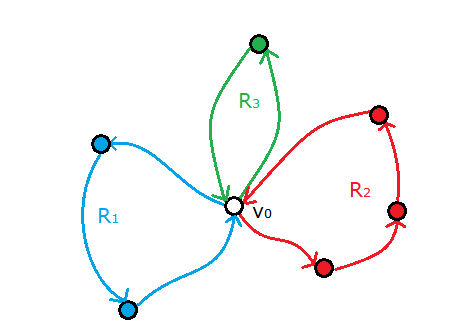
\includegraphics[width=0.5\textwidth]{figures/VRP_Szoveg_nelkul.png}
	\caption{Egy példa VRP végrehajtására n=7 csúcsú gráfon, k=3 járművel \label{VRPpelda} }
\end{figure}

\textbf{Matematikai megfogalmazás :} a problémát gráfokkal modellezhetjük.
\newline 
Legyen G = (V,E) (irányított) gráf, n az állomások száma (a kiindulási állomást beleértve), m az állomások között futó elérhető utak száma, k az elérhető járművek maximális száma.

\[ V = (v_0,v_1, \dots v_n )\]  állomások halmaza (Vertex), \(0 \in V\) a kiindulási állomás,
\[ E = (e_1,e_1, \dots e_m)\] elérhető utak halmaza (Edge),
\[ D : E(G) \mapsto \mathbb{Z}^+\] költségfüggvény (Distance),
\[ L = (l_1,l_2, \dots l_k)\] a járművek szállítási kapacitása (Load capacity),
\[ C : V(G)\setminus \{v_0\} \mapsto \mathbb{R}^+ \] az egyes állomások áruigénye (Claim),
\[ T_{min} :  V(G)\setminus \{v_0\} \mapsto \mathbb{R}^+ \] az egyes állomások készenléti ideje,
\[ T_{max} :  V(G)\setminus \{v_0\} \mapsto \mathbb{R}^+ \] az egyes állomások határideje. Értelemszerűen \(T_{max}(v_i) > T_{min}(v_i) \). A járművek sebessége 1 (tetszőleges egység), az idő és távolság egysége ugyanaz.

Az élek azonosítása érdekében éljünk a következő jelöléssel: e\textsubscript{ij} a v\textsubscript{i}-ből v\textsubscript{j}-be mutató él, és d\textsubscript{i,j} az e\textsubscript{i,j} költsége (itt : távolság, distance). Adott továbbá minden csúcshoz a c\textsubscript{i} áruigény, ami ki kell elégíteni (ez a valóságban lehet db, kg, stb.).Adott minden csúcshoz a c\textsubscript{i} áruigény, amit ki kell elégíteni (ez a valóságban lehet darab, kg, stb. ).  Legyen l\textsubscript{i} az i-edik jármű szállítási kapacitása.

Állítsuk elő útvonalak (Route) olyan \( R_{i} = (0, v_{i_1}, v_{i_2}, \dots 0) \) listáit,
ahol az i-edik jármű azon útvonalát adja meg, amelyet alkotó élek 
\( (e_{0,i_{1}}, e_{i_{1},i_{2}}, \dots e_{i_{m},0}) \). Az útvonal költsége az azt alkotó élek összköltsége. 
\begin{equation}
	c(R_i) = \sum_{v \in R_i} c(v)
\end{equation}


A cél azon \(R_1,R_2,...R_k \) útvonalak megtalálása, amelyekre a következők igazak:
\begin{itemize}
	\item összköltségük minimális
	\item kiindulási és végpontjuk a 0. állomás
	\item a kiindulási csúcsot leszámítva minden csúcsot pontosan egyszer tartalmaznak, vagyis \(\forall v_i \in V, v_i\ne v_0\) esetén \( \exists!R_j : v_i \in R_j \). 
	\item egyik jármű sem szállíthat több árut a megengedettnél, vagyis \(l_i \geqslant \sum_{v \in R_i} c(v) \)
	\item a járművek mindegyik állomásra időben megérkeznek: \(\forall v_i \in V, v_i\ne v_0\) esetén \( T_{min}(v_i) \leqslant t(v_i) \leqslant T_{max}(v_i) \)
\end{itemize}


\section{Hangyakolónia algoritmus \cite{alg_optim}}
A \ref{TSPsection}. és \ref{VRPsection}. fejezetekben ismertetett problémákra az optimális megoldás megtalálása NP-nehéz feladat, tahát nagy csúcs- és élhalmaz mellett nem gazdaságos az eredmény kiszámítása. Annak érdekében, hogy a gyakorlatban használható algoritmust konstruáljunk, valamilyen közelítő megoldást érdemes használni a direkt eljárások helyett. A hangyakolónia optimalizáció (Ant Colony Optimization - ACO) egy heurisztikus alapelv, mely gráfbejárások optimalizálásához képes gyorsan, az optimálishoz nagyon közeli megoldásokat biztosítani. Alkalmas a nagyfokú párhuzamosításra, ezért tökéletes választás az NVIDIA\textsuperscript{TM} CUDA architektúrájával történő, GPU alapú adaptálásra.

Az eljárás a nevéből adódóan a hangyák (Formicidae) természetben is megfigyelhető élelemkeresési módszerén alapszik. Az első felfedező hangyák véletlenszerű útvonalakon haladva keresik az élelemhez vezető utat, majd ha sikerrel jártak, akkor a visszaúton feromonnal jelölik meg az útjukat. A többi hangya a szagokat követi, ezért könnyebben, nagy számban tudnak eljutni az elemózsiához. Ha még maradt étel, ők is visszatérve erősítik a feromon nyomokat. Utánpótlás hiányában annak erőssége idővel gyengül, ami modellezhető exponenciális lecsengéssel. Ez természetes módon biztosítja, hogy a nem optimális útvonalak (az élelemhez vezet, de már van nála rövidebb) maguktól elhaljanak. Látható, hogy olyan él, ami sok ideig nem kap feromon utánpótlást, egyre kevesebb hangyát vonz.

Az algoritmus futása során nyilvántartunk egy az eredeti gráf topológiájával megegyező, de eltérő élsúlyozású feromongráfot. Legyen Ph(V,E) gráf, amiben az élek súlyai \( e_{i,j} \rightarrow \tau_{i,j} \) .

Gráfbejárás során egy \(v_i\)-n álló hangya a továbblépéséhez a lehetséges kimenő élek közül a feromon és és az élsúly alapján "céltábla elv szerint", véletlenszerűen választ. Úgy kell elképzelni, mintha egy beszínezett darts táblára dobálnánk, és a különböző színekhez az elérhető csúcsok tartoznak, a geometriai valószínűségi mező szerint kisebb-nagyobb valószínűségekkel. Az egyes élek kiválasztásának valószínűsége
\begin{equation}
	P_{i,j} = \frac{(\tau_{i,j})^\alpha(d_{i,j})^\beta}{\sum_{l \in N_i^k}(\tau_{i,l})^\alpha(d_{i,l})^\beta }
	\label{ACO_General_probability}
\end{equation}


ahol \(N_i^k \) az algoritmus k-adik lépésében az i-edik csúcsból elérhető szomszédos csúcsok halmaza. Az \(\alpha\) és \(\beta\) paraméterek a feromonok és élsúlyok figyelembevételét szabályozzák. A cél az, hogy minél nagyobb valahol a feromon, annál inkább akarjunk oda továbbmenni, illetve minél messzebb van egy adott pont, annál inkább el akarjuk kerülni. Saját megvalósításom esetében elhanyagoltam ezen ponton az élhosszak figyelembe vételét, ezért \(\beta = 0\). Továbbá az egyszerűség kedvéért legyen \(\alpha = 1\). Ennek az lesz az előnye, hogy a \ref{ACO_General_probability}. egyenlet nagymértékben leegyszerűsödik:
\begin{equation}
	P_{i,j} = \frac{\tau_{i,j}}{\sum_{l \in N_i^k}\tau_{i,l}}
	\label{ACO_My_probability}
\end{equation}

Miután minden hangya végigment egy úton (legeneráltunk egy csúcssorrendet, legyen az akár lehetséges, akár nem) értékeljük az útvonalakat. A teljesíthető útvonalak esetén a élek feromonszintjét a útvonal hosszával fordítottan arányosan \(\beta = -1\) megnövelem. Ez biztosítja, hogy a rövidebb útvonalak nagyobb feromonszinttel rendelkezzenek, ezáltal több hangya menjen előbb-utóbb olyan irányba. Valamilyen konstans szorzóra még szükség van a feromonértékek adott tartományba szabályozásához, ezért én még az addíciókat megszorzom a gráfban fellelhető átlagos bejárás hosszával. Így a hangsúly nem a konkrét hosszértékeken, hanem inkább az átlagoshoz vagy az optimálishoz viszonyított arányokon lesz.

Az éleken található feromon növelése után mindegyik élt exponenciális jelleggel csökkentem: minden feromon gyengül egy előre beállítandó, konstans szorzóval, ezzel veszem figyelembe a párolgást (\(\rho\)). Később úgy tapasztaltam, hogy egy \(\rho \approx 0.75\) választás megfelelőnek bizonyult. Összegezzük, hogy az egyes iterációk végén micsoda történik egy él feromonjával:
\[ \tau_{i,j} \leftarrow (1-\rho)\tau_{i,j} + \Delta\tau_{i,j} \]

Az útkeresés közben mindig fel kell jegyezni a legjobb addigi megtalált utat. Az ACO algoritmus egyik előnye, hogy több, hasonlóan jó alternatív utat is képes megtalálni. Ez például térképes útvonaltervezésnél lehet hasznos. Előfordulhat, hogy valami tőlünk független ok miatt a felhasználó egy objektíven nézve enyhén szuboptimális útvonalat akar inkább. Az eljárás javítása érdekében bevezettem, hogy az a hangya egy ún. "Jutalom szorzó"-t kap, aki minden korábbinál rövidebb utat talál. Ez azzal jár, a feromonjához adandó többlet a sokszorosára, pélául százszorosára változik, így a következő iterációban sokkal nagyobb valószínűséggel fog arra menni a jövő hangyája. A jutalmazási rendszerem rossz beállítások mellett kezdetben félreviheti a hangyákat egy szuboptimális, de lokálisan minimális útvonal felé. Ha ilyen jelenség tapasztalható, akkor át lehet állítani, hogy hányadik iterációtól kezdve kaphassanak az útvonalak "Jutalom szorzó"-t.

Az eljárás adott számú iteráció után leáll, az eredmény lehetőleg az addig megtalált legrövidebb útvonal. A konkrét implementáció során látni fogjuk, hogy a helyzet bonyolódhat. \textcolor{red}{UTALÁS}

%TODO UTALÁS

\section{Alternatív megoldások}

Dolgozatomban főleg a Hangyakolónia algoritmussal foglalkoztam, de  az nem azt jelenti, hogy ez az egyetlen járható út. Nézzünk meg néhány alternatív kiindulási gondolatot.

\subsection{„Brute force” algoritmus}
A „Brute force” algoritmus lényege, hogy minden lehetséges bejárást megvizsgálunk, és kiválasztjuk a legrövidebb, a konkrét probléma feltétel(rendszer)ének eleget tevő esetet. \textbf{Ha n db csúcs}ból álló teljes gráfot nézünk, mint ahogy az a valóságban igen gyakori, \textbf{akkor n! különböző lehetséges bejárás}t kell összehasonlítani. Kis n esetén még csak-csak elfogadható ez a módszer, viszont ha már \(n=48\) db csúcsunk van, mert szeretnénk bejárni TSP szerint az Amerikai Egyesült Államok 48 összefüggő államának fővárosait (később lesz rá példa), a vizsgálandó esetek száma felugrik \( 48! \approx 1.24 * 10^{61} \)-re. Tegyük fel, hogy csúcskategóriás, 5 GHz-en pörgő szuperszámítógépünk képes átlagosan 1 órajelciklusonként (  \(2*10^{-10}s\) időközönként, nagyjából lehetetlenül gyorsan) kiszámolni egy út hosszát, még így is kb. \(2.5 * 10^{51}s \approx 8 * 10^{43} \) évig vizsgálhatnánk az eseteket. Egy SMD beültetőgép a szerelőlemezre akár alkatrészek százait pakolhatja fel, brute force módszerrel lehetetlen lenne megmondani, hogy milyen sorrendben haladjon. Ha szeretnénk véges időn belül megoldani a problémát, márpedig szeretnénk, akkor ravaszabbnak kell lennünk.

\subsection{Held - Karp algoritmus }
A Held-Karp algoritmust M. Held és R. Karp urak alkották meg 1962-ben \cite{HeldKarp}. Akkoriban még csak gyerekcipőben a számítástudomány és az informatika, ekkor készültek el az első számítógépek. Módszerük szerint egyesével, rendezetten szúrnak be csúcsokat egy egyre növekvő ponthalmazba. Hasonlít a beillesztéses rendezésre, csak kicsit komplexebb. Kihasználja, hogy a stack (magyarul: verem) és a stackpointer megjelenésével a korai számítógépek is képesek voltak már rekurzív programvégrehajtásra.
\paragraph{}
Jelöljük a csúcsokat \( V=\left(v_1,v_2,\ldots v_n\right) \) -nel, \(v_1\) önkényesen kijelölhető kezdőpontnak. Legyen S halmaz a csúcsok valamely, a kezdőcsúcsot nem tartalmazó részhalmaza: \(S \subseteq \{v_2,...v_n\}\). Legyen g(S,e) \(v_1\)-ből az S összes elemén keresztül az e \(\neq v_1\)  csúcsba végződő legrövidebb út hossza. Az u-ból a v-be mutató él költsége d(u,v).
Lépésenként kiszámítjuk a g(S,e) értékeket kezdte a kis S-ekre.

Példák:
\begin{itemize}
	\item \(\forall e: g(\emptyset,e) = d(1,e)\)
	\item \(g(\{2\},4)\) csak az összhossza az  \(1 \rightarrowtail 2 \rightarrowtail 4\) útnak
	\item \(g(\{2,3\},4)\)  az ( \(1 \rightarrowtail 2 \rightarrowtail 3 \rightarrowtail 4\) ) és ( \(1 \rightarrowtail 3 \rightarrowtail 2 \rightarrowtail 4\) ) utak rövidebbikének a költsége
\end{itemize}

Amikor már 3 vagy több pontot tartalmaz az S halmaz, a lehetséges utak száma drasztikusan megnő, de egy ügyes trükk felhasználásával csak néhányat kell figyelembe venni a legrövidebb út keresése érdekében. Vegyük észre, hogyha az (\(1\rightarrowtail 4\rightarrowtail 3\rightarrowtail 2\)) út rövidebb, mint az (\(1\rightarrowtail 3\rightarrowtail 4\rightarrowtail 2\)), akkor az (\(1\rightarrowtail 4\rightarrowtail 3\rightarrowtail 2\rightarrowtail 5\)) út is rövidebb lesz, mint a (\(1\rightarrowtail 3\rightarrowtail 4\rightarrowtail 2\rightarrowtail 5\)).
\paragraph{}
Általánosan: tegyük fel, hogy a k-adik lépésben \(S=\{s_1,...s_k\}\). Jelöljük \(1\leqslant i\leqslant k\)-ra \(S_i = S-\{s_i\} = \{s_1...s_{i-1},s_{i+1}...s_k\} \). Ha a \(v_1\)-ből a legrövidebb út e-be S-en keresztül úgy vezet, hogy annak \(s_i\) az utolsó előtti eleme, akkor következik, hogy \(v_1\)-ből a legrövidebb út \(s_i\)-be \(S_i\)-n keresztül vezet. Ez azt jelenti, hogy a k-adik lépésben elég k db S halmazt továbbvinnünk, mert csak azok lehetségesek legrövidebb utat adni.

\subsubsection{Az eljárás Értékelése}
A Held-Karp algoritmus exponenciális idejű, \(O(2^nn^2)\), ami nagyságrendekkel jobb, mint a brute-force módszer az ő \(O(n!)\) faktoriális idejével. Előnye a Hangyakolónia algoritmussal szemben, hogy determinisztikus algoritmus révén a végén mindig a legrövidebb utat adja eredményül. Komoly hátránya, hogy rekurziót alkalmaz, ami kedvezőtlen a programvégrehajtás szempontjából: sok rekurzív függvényhívás ugyanis megterheli a stacket, sok felesleges másolás történik. Belátható, hogy ha különböző, adott esetekben bonyolult feltételekkel keresünk utakat, akkor az algoritmus elveszíti alapelvét, nem elég mindig az előző ciklus legjobbjaiból kiindulni. Ezzel a problémával az ACO is szembesül, de kevésbé van rá kihatással. Erre még később visszatérünk a \textcolor{red}{UTALÁS} \ref{CVRPTWsection} fejezetben, ahol a feltételek bonyolódásával foglalkozom.

%TODO UTALÁS